\documentclass[12pt]{book}

\usepackage[paperwidth=4.5in, paperheight=7in]{geometry}
\usepackage{graphicx}
\usepackage{parskip}
\usepackage{titlesec}
\usepackage{color}
\usepackage{subcaption}

\definecolor{on}{RGB}{28, 113, 17}
\definecolor{off}{RGB}{233, 19, 19}
\definecolor{unknown}{RGB}{67, 107, 204}

\brokenpenalty 10000

\frenchspacing

\newcommand{\ON}{\textcolor{on}{ON}}
\newcommand{\OFF}{\textcolor{off}{OFF}}

\titleformat{\chapter}[display]{\normalfont\huge\bfseries}{}{0pt}{\Huge}\titlespacing*{\chapter}{0pt}{-50pt}{20pt}

\title{
\includegraphics[width=\textwidth]{GameLogo}}
\author{Vincent Macri \and Chloe Nguyen \and Susie Son}
\date{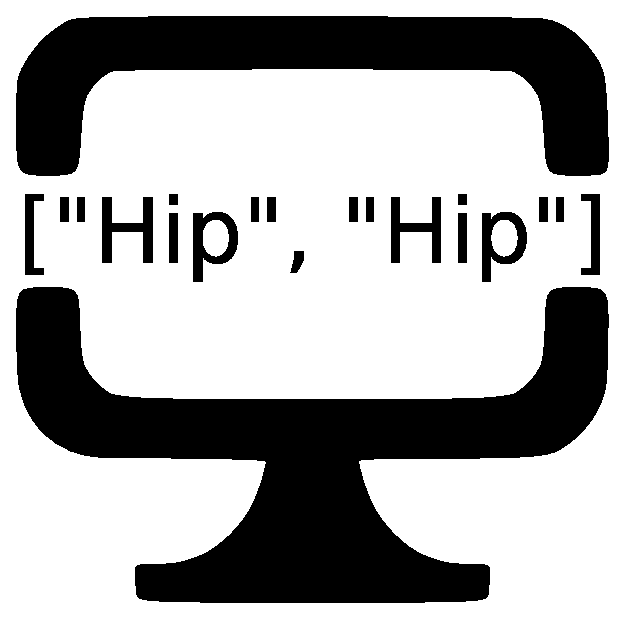
\includegraphics[width=0.5\textwidth]{CompanyLogo}\\\copyright 2017 Hip Hip Array}

\begin{document}
	\pagenumbering{gobble}
	\maketitle
	\begingroup
		\let\cleardoublepage\clearpage
		\frontmatter
		\tableofcontents
		\mainmatter
	\endgroup
	\chapter{The Story}
		You are the world's best ICS teacher, Ms. Krasteva. As a thank you gift for an amazing year of teaching, your students bought you a coffee. But when you drink the coffee, you start to feel funny.

		When you get home, you turn on your TV, and start to watch the news. They are running a story on a coffee recall! Due to horrible quality control, coffee from Starbucks is turning people sick. But not just a normal kind of sick. It is turning them into mice!

		You see the world around you getting bigger, but it isn't. Ms. Krasteva is turning into Mouse Krasteva!

		The news wrapped up the story by mentioning that the company ``Hip Hip Array'' is testing an antidote. However, you do not have time to wait for this antidote, because you need to mark the fantastic ISPs your students have poured the last month of their lives into in an effort to get 100%.

		You take it upon yourself to break into the lab and steal the antidote because mice are unable to use computer mice.

		Unfortunately for you, the lab has a high-tech security system of boolean algebra mazes and cat security guards, meaning that you have to avoid getting electrocuted while collecting fish to bribe the cats to not to eat you.
		\begin{center}
			
\includegraphics[width=0.4\textwidth]{Cat}
			\hspace{5mm}
			
\includegraphics[width=0.4\textwidth]{Mouse}
		\end{center}
	\chapter{Main Menu}
		The menu provides you with a few options:
		\begin{description}
			\item[Play] Click this button to play the game. The game will continue from where you left off.
			\item[Help] Click this button to learn how to play the game.
			\item[High Scores] Click this button to see the high scores.
			\item[Settings] Click this button to change the game settings.
			\item[Credits] Click this button to see the game credits.
			\item[License] Click this button to view the copyright notice.
			\item[Quit] Click this button to close the game.
		\end{description}
		\newpage
		\vspace*{\fill}
		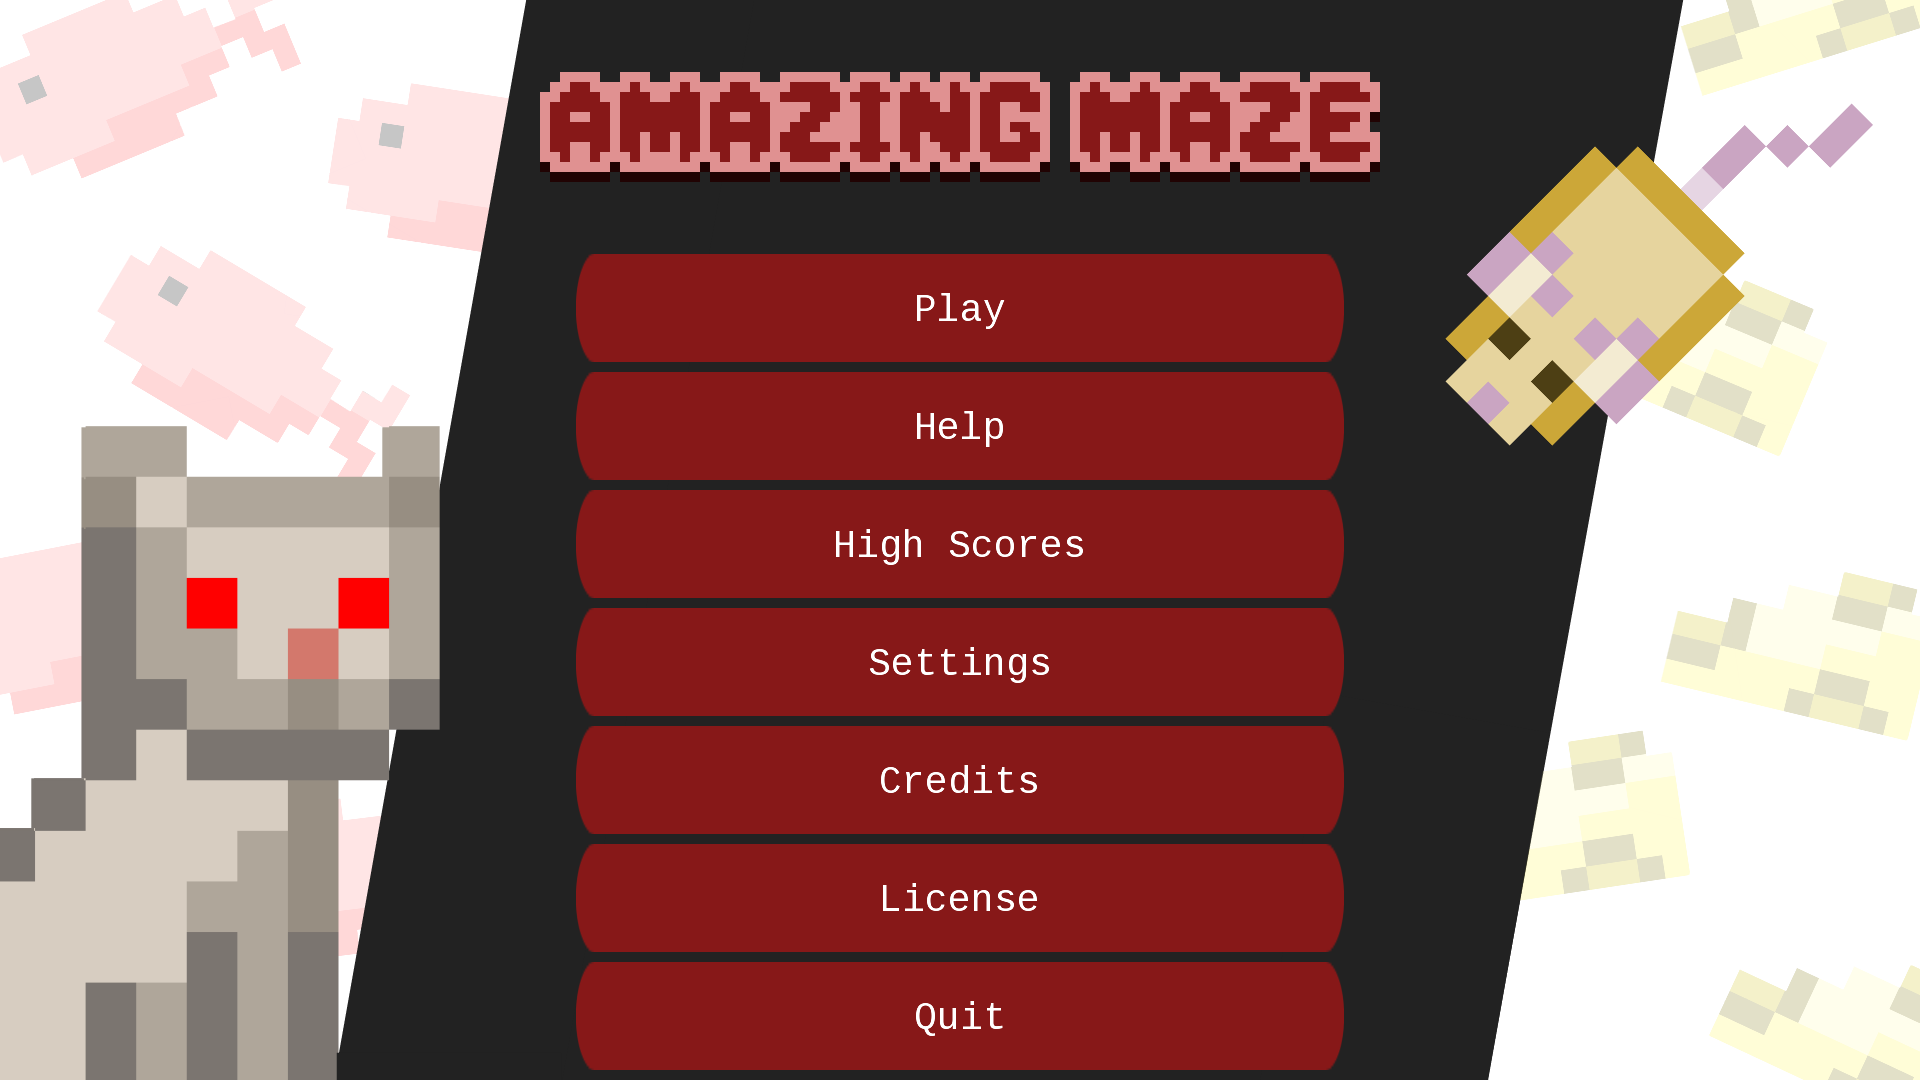
\includegraphics[width=\textwidth]{MainMenu}
		\vspace*{\fill}
	\chapter{Settings}
		On the settings menu, you are able to:
		\begin{itemize}
			\item Adjust the volume level
			\item Change the controls
			\item Reset the settings
			\item Reset your save file
		\end{itemize}
		\newpage
		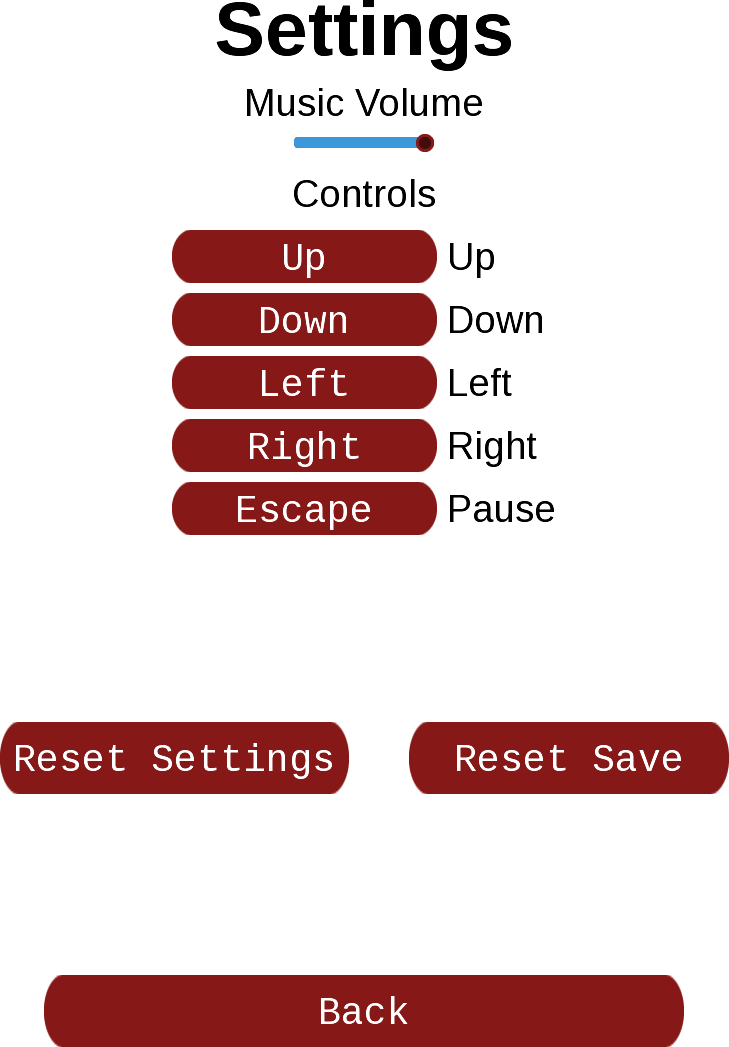
\includegraphics[width=\textwidth]{SettingsScreen}
	\chapter{Maze}
		\section{Maze Screen}
			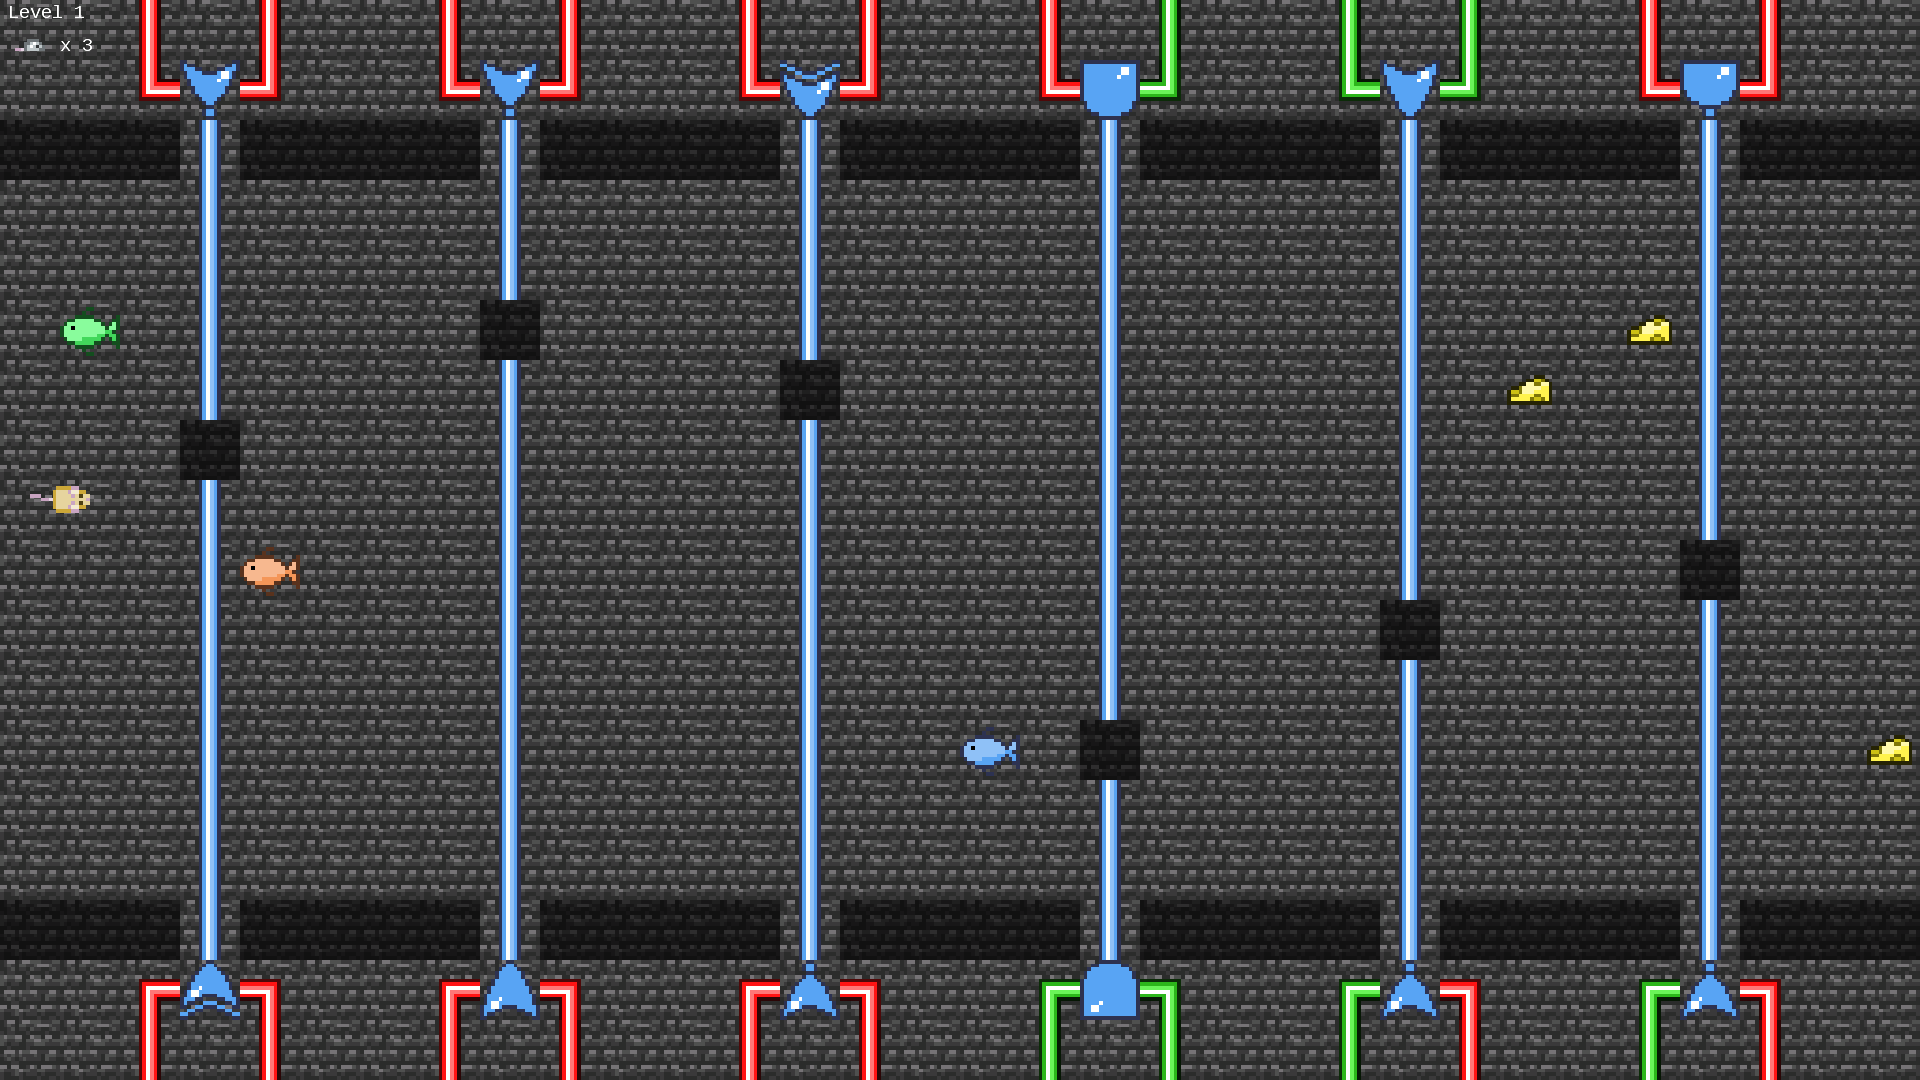
\includegraphics[width=\textwidth]{MazeScreen}
			\\
			Here we see the mouse (on the left, in the middle of the screen) at the start of a new level.

			In the top left, we see that the player has three lives remaining.
		\section{Goal}
			In the maze, you must navigate through logic gates.

			Each gate has two inputs, and one output.
			\\
			\textcolor{on}{Green is on, or true.}
			\\
			\textcolor{off}{Red is off, or false.}
			\\
			\textcolor{unknown}{Blue is unknown.}

			\begin{figure}[h]
				\centering
				\begin{subfigure}[t]{0.3\textwidth}
					\centering
					
\includegraphics[width=0.3\textwidth]{ON}

					An on wire.
				\end{subfigure}
				\hspace{1mm}
				\begin{subfigure}[t]{0.3\textwidth}
					\centering
					
\includegraphics[width=0.3\textwidth]{OFF}

					An off wire.
				\end{subfigure}
				\hspace{1mm}
				\begin{subfigure}[t]{0.3\textwidth}
					\centering
					
\includegraphics[width=0.3\textwidth]{UNKNOWN}

					An unknown wire.
				\end{subfigure}
			\end{figure}

			The two inputs will always be known, and \emph{you} will always need to determine the output.

			You will be working with AND, NAND, OR, NOR, and XOR gates.
		\section{AND Gate}
			An AND gate is on only if both of its inputs are on.
			\begin{figure}[h]
				\centering
				\begin{subfigure}{0.75\textwidth}
					\begin{tabular}{|c|c|c|}
						\hline
						\textbf{Input A} & \textbf{Input B} & \textbf{Output}\\\hline
						\OFF & \OFF & \OFF\\\hline
						\OFF & \ON & \OFF\\\hline
						\ON & \OFF & \OFF\\\hline
						\ON & \ON & \ON\\\hline
					\end{tabular}
				\end{subfigure}
				\begin{subfigure}{0.2\textwidth}
					\centering
					
\includegraphics[width=0.75\textwidth]{AND}
				\end{subfigure}
			\end{figure}
		\vspace{-20pt}
		\section{NAND Gate}
			A NAND gate's output is the opposite of an AND gate's with the same inputs. It is a \emph{not} AND gate.
			\begin{figure}[h]
				\centering
				\begin{subfigure}{0.75\textwidth}
					\begin{tabular}{|c|c|c|}
						\hline
						\textbf{Input A} & \textbf{Input B} & \textbf{Output}\\\hline
						\OFF & \OFF & \ON\\\hline
						\OFF & \ON & \ON\\\hline
						\ON & \OFF & \ON\\\hline
						\ON & \ON & \OFF\\\hline
					\end{tabular}
				\end{subfigure}
				\begin{subfigure}{0.2\textwidth}
					\centering
					
\includegraphics[width=0.75\textwidth]{NAND}
				\end{subfigure}
			\end{figure}
		\section{OR Gate}
			An OR gate is on if at least of its inputs are on.
			\begin{figure}[h]
				\centering
				\begin{subfigure}{0.75\textwidth}
					\begin{tabular}{|c|c|c|}
						\hline
						\textbf{Input A} & \textbf{Input B} & \textbf{Output}\\\hline
						\OFF & \OFF & \OFF\\\hline
						\OFF & \ON & \ON\\\hline
						\ON & \OFF & \ON\\\hline
						\ON & \ON & \ON\\\hline
					\end{tabular}
				\end{subfigure}
				\begin{subfigure}{0.2\textwidth}
					\centering
					
\includegraphics[width=0.75\textwidth]{OR}
				\end{subfigure}
			\end{figure}
		\vspace{-20pt}
		\section{NOR Gate}
			A NOR gate's output is the opposite of an OR gate's with the same inputs. It is a \emph{not} OR gate.
			\begin{figure}[h]
				\centering
				\begin{subfigure}{0.75\textwidth}
					\begin{tabular}{|c|c|c|}
						\hline
						\textbf{Input A} & \textbf{Input B} & \textbf{Output}\\\hline
						\OFF & \OFF & \ON\\\hline
						\OFF & \ON & \OFF\\\hline
						\ON & \OFF & \OFF\\\hline
						\ON & \ON & \OFF\\\hline
					\end{tabular}
				\end{subfigure}
				\begin{subfigure}{0.2\textwidth}
					\centering
					
\includegraphics[width=0.75\textwidth]{NOR}
				\end{subfigure}
			\end{figure}
		\section{XOR Gate}
			An XOR gate is on if only one of its inputs are on.
			\begin{figure}[h]
				\centering
				\begin{subfigure}{0.75\textwidth}
					\begin{tabular}{|c|c|c|}
						\hline
						\textbf{Input A} & \textbf{Input B} & \textbf{Output}\\\hline
						\OFF & \OFF & \OFF\\\hline
						\OFF & \ON & \ON\\\hline
						\ON & \OFF & \ON\\\hline
						\ON & \ON & \OFF\\\hline
					\end{tabular}
				\end{subfigure}
				\begin{subfigure}{0.2\textwidth}
					\centering
					
\includegraphics[width=0.75\textwidth]{XOR}
				\end{subfigure}
			\end{figure}
		\vspace{-20pt}
		\section{Interacting with Gates}
			The goal of this game is to reach the right side of the map without touching any wires that are on. While not necessary, you make click on the gates to mark them with what you think their output is. Left click a gate to mark it as on. Right click a gate to mark it as off. Middle click a gate to mark it as unknown.
		\section{Items}
			\subsection{Fish}
				There are 5 fish you can collect in the game, each worth a different amount of points corresponding to Canadian money. Collecting these fish is what gets you points.
				\begin{figure}[h]
					\centering
					\begin{subfigure}[t]{0.16\textwidth}
						\centering
						
\includegraphics[width=\textwidth]{BlueFish}
						5
					\end{subfigure}
					\hspace{1mm}
					\begin{subfigure}[t]{0.16\textwidth}
						\centering
						
\includegraphics[width=\textwidth]{PurpleFish}
						10
					\end{subfigure}
					\hspace{1mm}
					\begin{subfigure}[t]{0.16\textwidth}
						\centering
						
\includegraphics[width=\textwidth]{GreenFish}
						20
					\end{subfigure}
					\hspace{1mm}
					\begin{subfigure}[t]{0.16\textwidth}
						\centering
						
\includegraphics[width=\textwidth]{RedFish}
						50
					\end{subfigure}
					\hspace{1mm}
					\begin{subfigure}[t]{0.16\textwidth}
						\centering
						
\includegraphics[width=\textwidth]{OrangeFish}
						100
					\end{subfigure}
				\end{figure}
			\subsection{Cheese}
				Because you are a mouse, cheese is incredibly healthy. Eating cheese will give you more lives.
				\begin{center}
					
\includegraphics[width=0.35\textwidth]{Cheese}
				\end{center}
	\chapter{Counting Points}
		You count your points manually. A sketchpad is provided for you to do your work on.

		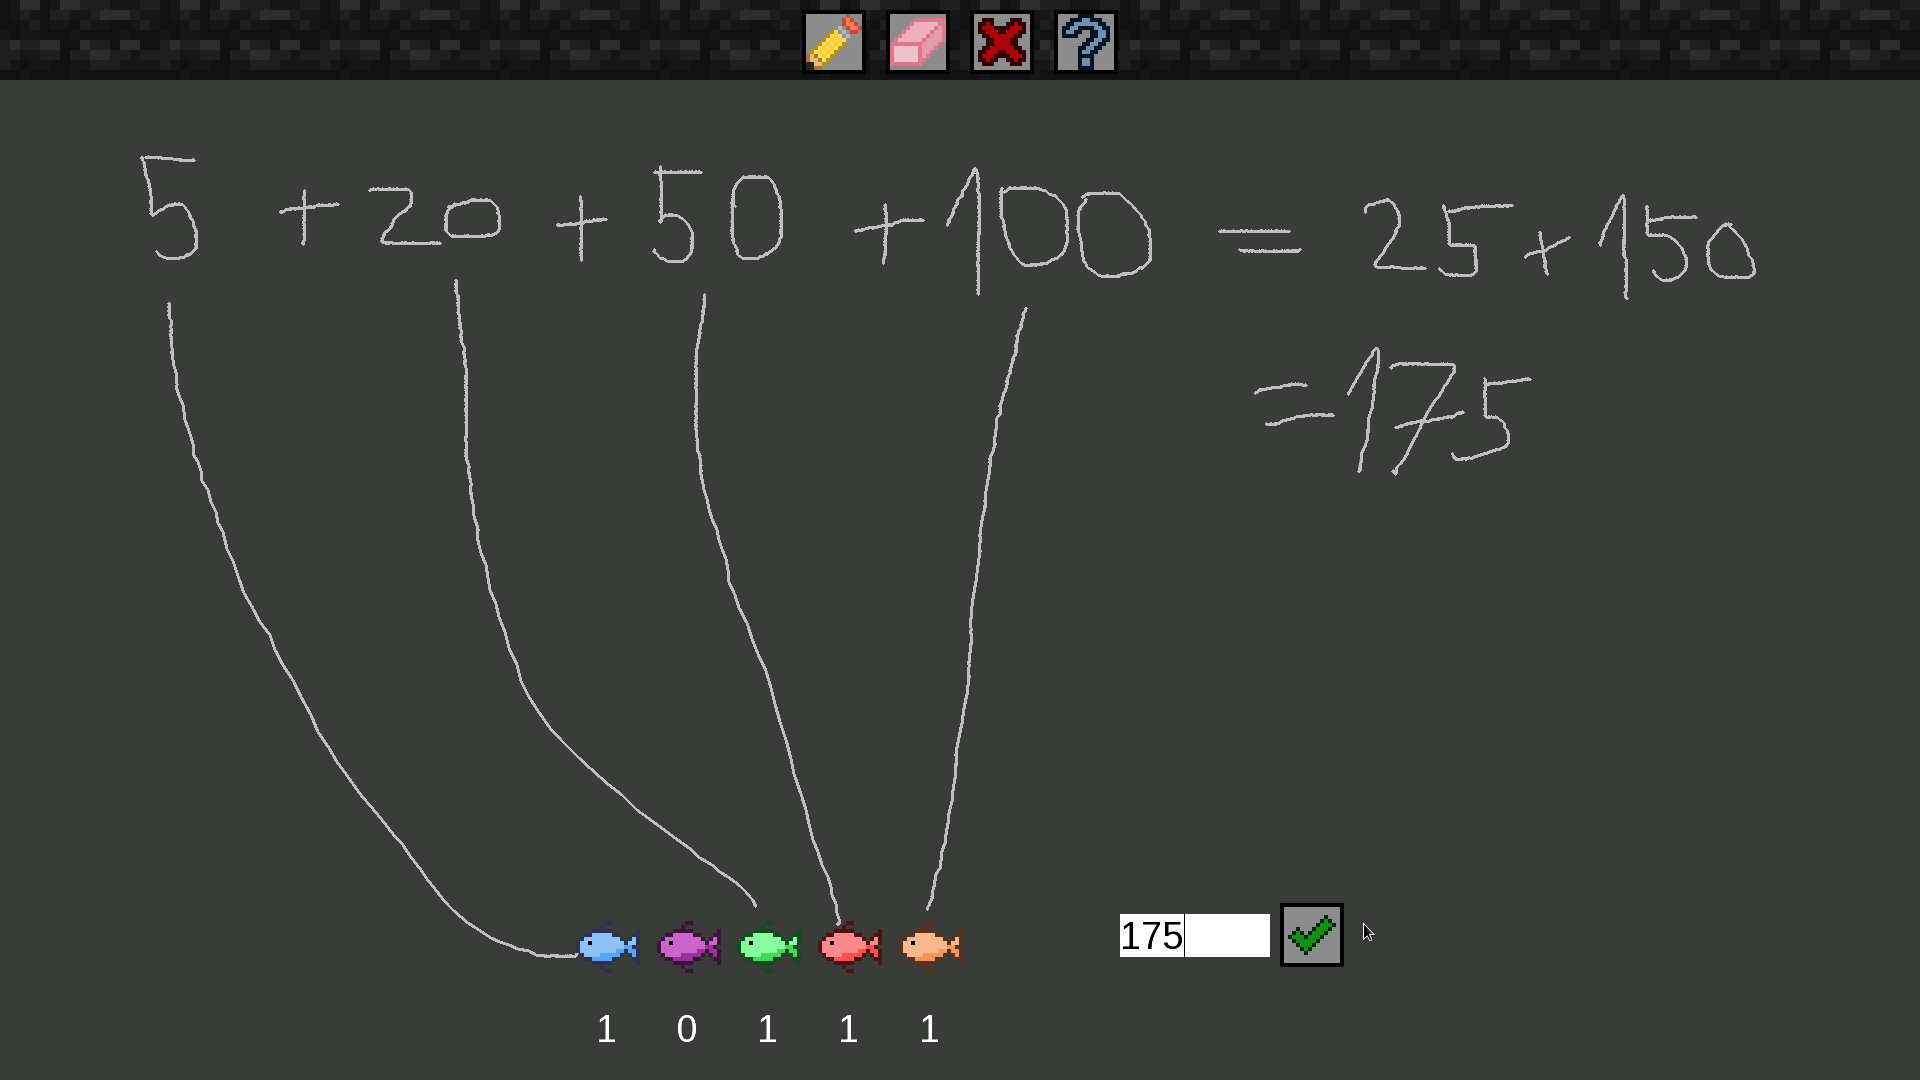
\includegraphics[width=\textwidth]{CountingScreen}

		This example shows how you might count up your score on the screen and input the answer.

		The closer you are to the correct answer, the more points you will get. There is a help button on this screen which reminds you how many points each item is worth.
		\section{Controls}
			Click 
\includegraphics[height=\baselineskip]{Pencil} to enter drawing mode. Click 
\includegraphics[height=\baselineskip]{Eraser} to enter erasing mode. The screen starts in drawing mode.

			If you make a big mistake, click 
\includegraphics[height=\baselineskip]{Clear} to erase everything.

			Once you think you have the correct answer, click 
\includegraphics[height=\baselineskip]{Check} to submit it.

			If you forget how this part of the game works, click 
\includegraphics[height=\baselineskip]{Help} for a reminder of the rules.
		\section{Scoring}
			If you count your score correctly, you get all of the points. If you are off by 1-5, you get 70\% of the points. If you are off by 6-15, you get 50\% of the points. If you are off by more than 15, you get 15\% of the points.
\end{document}
